\section{Mapping The Effects of Reward Misspecification}\label{app:measurement}

\begin{figure}[!h]
\centering
\subfloat[\label{fig:t_mis_merge}\textit{traffic\_merge} - Misweighting] {\includegraphics[scale=0.60]{figures/traffic/accel_max_proxy_single.eps}}%
\hfill
\subfloat[\label{fig:t_ont_bottle}\textit{traffic\_bottle} - Misweighting] {\includegraphics[scale=0.60]{figures/traffic/bottle_max_proxy_single.eps}}%
\vfill
\subfloat[\label{fig:t_space_merge}\textit{traffic\_merge} - Space] {\includegraphics[scale=0.60]{figures/traffic/space_max_proxy_single.eps}}%
\hfill
\subfloat[\label{fig:p_mis}COVID - Misweighting] {\includegraphics[scale=0.60]{figures/pandemic/misweight_max_proxy_single.eps}}%
\vfill
\subfloat[\label{fig:a_ont}Atari - Ontological] {\includegraphics[scale=0.60]{figures/atari/pacifist_max_proxy_single.eps}}%
\hfill
\subfloat[\label{fig:a_mis}Atari - Misweighting] {\includegraphics[scale=0.60]{figures/atari/move_max_proxy_single.eps}}%


\caption{Additional model size scatter plots. Observe that not all misspecifications cause misalignment. We plot the \textcolor{bluetext}{proxy reward} with ``$\bullet$" and the \textcolor{greentext}{true reward} with ``$\times$". The proxy reward is measured on the left-hand side of each figure and the true reward is measured on the right hand side of each figure.}
\label{fig:modelsize_scatter_appendix}
\end{figure}
\subsection{Effect of Model Size}\label{app:modelsize_plots}
We plot the proxy and true reward vs. model size in Figure~\ref{fig:modelsize_scatter_appendix}, following the experiment described in Section~\ref{sec:quantitative}.
\newpage

\begin{figure}[!ht]
\centering
\subfloat[\label{fig:corr_bottle_1}\textit{traffic\_bottle} - Misweighting] {\includegraphics[scale=0.62]{figures/traffic/bottle_max_proxy_single.eps}}%
\hfill
\subfloat[\label{fig:corr_bottle_2}Correlation for Figure~\ref{fig:corr_bottle_1}] {\includegraphics[scale=0.62]{figures/correlation/bottle_correlation.eps}}%

\subfloat[\label{fig:corr_accel_1}\textit{traffic\_merge} - Misweighting] {\includegraphics[scale=0.62]{figures/traffic/accel_max_proxy_single.eps}}%
\hfill
\subfloat[\label{fig:corr_accel_2}Correlation for Figure~\ref{fig:corr_accel_1}] {\includegraphics[scale=0.62]{figures/correlation/accel_correlation.eps}}%

\subfloat[\label{fig:corr_bus_1}\textit{traffic\_merge} - Ontological] {\includegraphics[scale=0.62]{figures/traffic/commute_max_proxy_single.eps}}%
\hfill
\subfloat[\label{fig:corr_bus_2}Correlation for Figure~\ref{fig:corr_bus_1}] {\includegraphics[scale=0.62]{figures/correlation/bus_correlation.eps}}%


\caption{Correlations between the proxy and true rewards, along with the reward hacking induced. In the left column, we plot the \textcolor{bluetext}{proxy reward} with ``$\bullet$" and the \textcolor{greentext}{true reward} with ``$\times$". In the right column, we plot the \textcolor{purpletext}{trained checkpoint correlation} and the \textcolor{yellowtext}{randomly initialized checkpoint correlation}.}
\label{fig:correlation_appendix}
\end{figure}

\subsection{Correlation between Proxy and True Rewards}\label{app:measurement_correlation}
We plot the correlation between proxy and true rewards, following the experiment described in Section~\ref{sec:correlation}. Interestingly, we see that reward hacking still occurs when there is positive correlation between the true and proxy rewards, e.g., in Figures~\ref{fig:corr_bottle_1}/\ref{fig:corr_bottle_2}. Unsurprisingly, proxy-true pairs which are highly correlated, e.g., Figure~\ref{fig:corr_accel_1}/\ref{fig:corr_accel_2} do not exhibit reward hacking. Finally, proxy-true pairs which are negatively correlated, e.g., Figure~\ref{fig:corr_bus_1}/\ref{fig:corr_bus_2} exhibit the most reward hacking. 


% \textbf{Traffic.}
% For the \textit{misweighting} misspecification, we work with the \textit{traffic-merge} setup (see Section~\ref{sec:environments}). The proxy reward function downweights the penalty for accelerating. As a result, the agent causes the AVs to frequently accelerate and decelerate, producing waves in the traffic. Although this leads to a high average speed, the waves imply frequent acceleration, which has low true reward. Furthermore, actually driving in the waves is less pleasant than driving in smoother traffic.

% For the \textit{ontological misspecification}, we work with the \textit{traffic-bottleneck} setup (see Section~\ref{sec:environments}). AVs and human drivers are driving on a highway whose lanes are progressively reduced to one. The proxy reward function rewards high average velocity, whereas the true reward function rewards the outflow rate (number of cars leaving the bottleneck). More capable policies learn to increase the velocity by accelerating the AVs before the bottleneck. However, the AVs then create greater congestion near the bottleneck and reduce outflow.

% \textbf{COVID.} For \textit{misweighting} misspecification, the proxy reward function upweights the relative importance of the public health relative to the economic health. Intuitively, one would expect more capable models to overemphasize public health, and therefore maintain the regulations at higher levels than desired. However, because the number of infections increase exponentially, raising the stage at earlier stages of the pandemic is more effective. In this case, both economic and public desiderata are well-aligned, so optimizing for one objective also improves the other.


% \textbf{Effect of training steps}

% Reward hacking vs. training steps: same as above (possibly defer this or others to appendix if we run out of space)
\newpage